\documentclass[11pt]{article}
\usepackage[textwidth=18.0cm, textheight=23.0cm, top=2.0cm]{geometry}
\usepackage{pst-all}
\usepackage{amssymb}
\usepackage{tikz}
\usepackage{underscore}\begin{document}
\pagestyle{empty}


ClassName: \underline{\textbf{Class_02.2bp-17}}
\par
BinSize: \underline{\textbf{30 × 30}}
\par
ReduceSize: \underline{\textbf{30 × 30}}
\par
TypeNum: \underline{\textbf{35}}
\par
Num: \underline{\textbf{40}}
\par
OutS: \underline{\textbf{1800}}
\par
InS: \underline{\textbf{1454}}
\par
Rate: \underline{\textbf{0.808}}
\par
UB: \underline{\textbf{2}}
\par
LB0: \underline{\textbf{2}}
\par
LB: \underline{\textbf{2}}
\par
LBWithCut: \underline{\textbf{2}}
\par
NodeCut: \underline{\textbf{0}}
\par
ExtendedNodeCnt: \underline{\textbf{1}}
\par
GenNodeCnt: \underline{\textbf{1}}
\par
PrimalNode: \underline{\textbf{0}}
\par
ColumnCount: \underline{\textbf{2}}
\par
TotalCutCount: \underline{\textbf{0}}
\par
RootCutCount: \underline{\textbf{0}}
\par
LPSolverCnt: \underline{\textbf{1}}
\par
PricingSolverCnt: \underline{\textbf{0}}
\par
BranchAndBoundNum: \underline{\textbf{1}}
\par
isOpt: \underline{\textbf{true}}
\par
TimeOnPrimal: \underline{\textbf{0.000 s}}
\par
TimeOnPricing: \underline{\textbf{0.000 s}}
\par
TimeOnRmp: \underline{\textbf{0.063 s}}
\par
TotalTime: \underline{\textbf{0.110 s}}
\par
\newpage


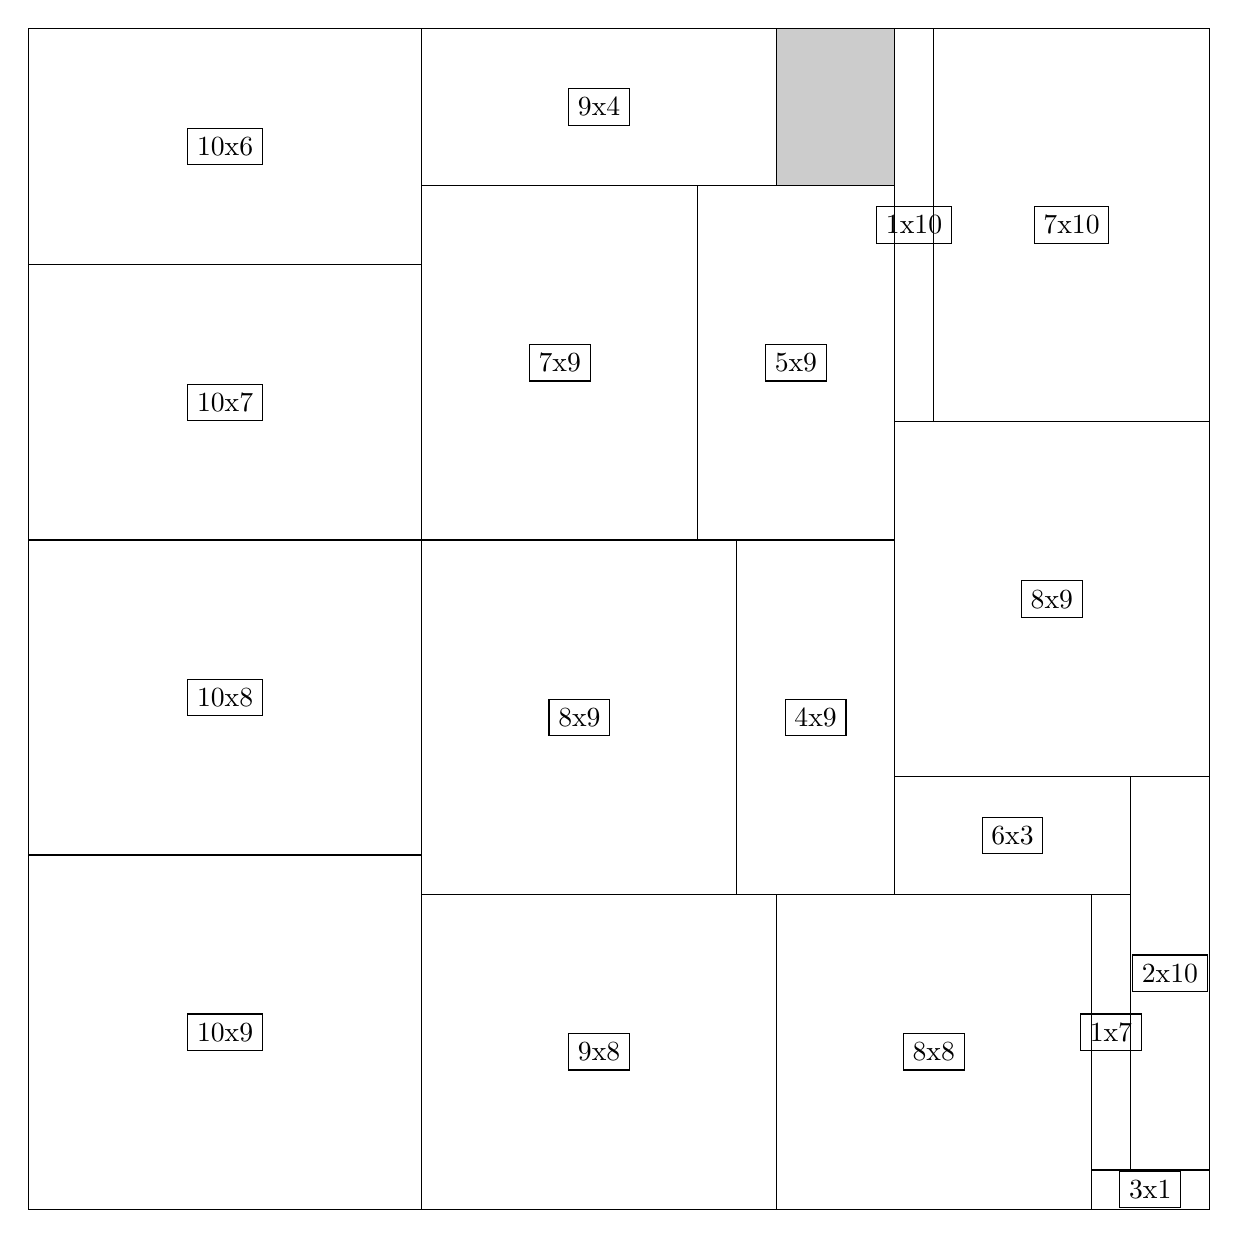
\begin{tikzpicture}[shorten >=1pt,scale=1.0,every node/.style={scale=1.0},->]
\tikzstyle{vertex}=[circle,fill=black!25,minimum size=14pt,inner sep=0pt]
\filldraw[fill=gray!40!white, draw=black] (0,0) rectangle (15.0,15.0);
\foreach \name/\x/\y/\w/\h in {10x9/0.0/0.0/5.0/4.5,10x8/0.0/4.5/5.0/4.0,9x8/5.0/0.0/4.5/4.0,8x9/11.0/5.5/4.0/4.5,8x9/5.0/4.0/4.0/4.5,10x7/0.0/8.5/5.0/3.5,7x10/11.5/10.0/3.5/5.0,8x8/9.5/0.0/4.0/4.0,7x9/5.0/8.5/3.5/4.5,10x6/0.0/12.0/5.0/3.0,5x9/8.5/8.5/2.5/4.5,9x4/5.0/13.0/4.5/2.0,4x9/9.0/4.0/2.0/4.5,2x10/14.0/0.5/1.0/5.0,6x3/11.0/4.0/3.0/1.5,1x10/11.0/10.0/0.5/5.0,1x7/13.5/0.5/0.5/3.5,3x1/13.5/0.0/1.5/0.5}
\filldraw[fill=white!40!white, draw=black] (\x,\y) rectangle node[draw] (\name) {\name} ++(\w,\h);
\end{tikzpicture}


w =10 , h =9 , x =0 , y =0 , v =90
\par
w =10 , h =8 , x =0 , y =9 , v =80
\par
w =9 , h =8 , x =10 , y =0 , v =72
\par
w =8 , h =9 , x =22 , y =11 , v =72
\par
w =8 , h =9 , x =10 , y =8 , v =72
\par
w =10 , h =7 , x =0 , y =17 , v =70
\par
w =7 , h =10 , x =23 , y =20 , v =70
\par
w =8 , h =8 , x =19 , y =0 , v =64
\par
w =7 , h =9 , x =10 , y =17 , v =63
\par
w =10 , h =6 , x =0 , y =24 , v =60
\par
w =5 , h =9 , x =17 , y =17 , v =45
\par
w =9 , h =4 , x =10 , y =26 , v =36
\par
w =4 , h =9 , x =18 , y =8 , v =36
\par
w =2 , h =10 , x =28 , y =1 , v =20
\par
w =6 , h =3 , x =22 , y =8 , v =18
\par
w =1 , h =10 , x =22 , y =20 , v =10
\par
w =1 , h =7 , x =27 , y =1 , v =7
\par
w =3 , h =1 , x =27 , y =0 , v =3
\par
\newpage


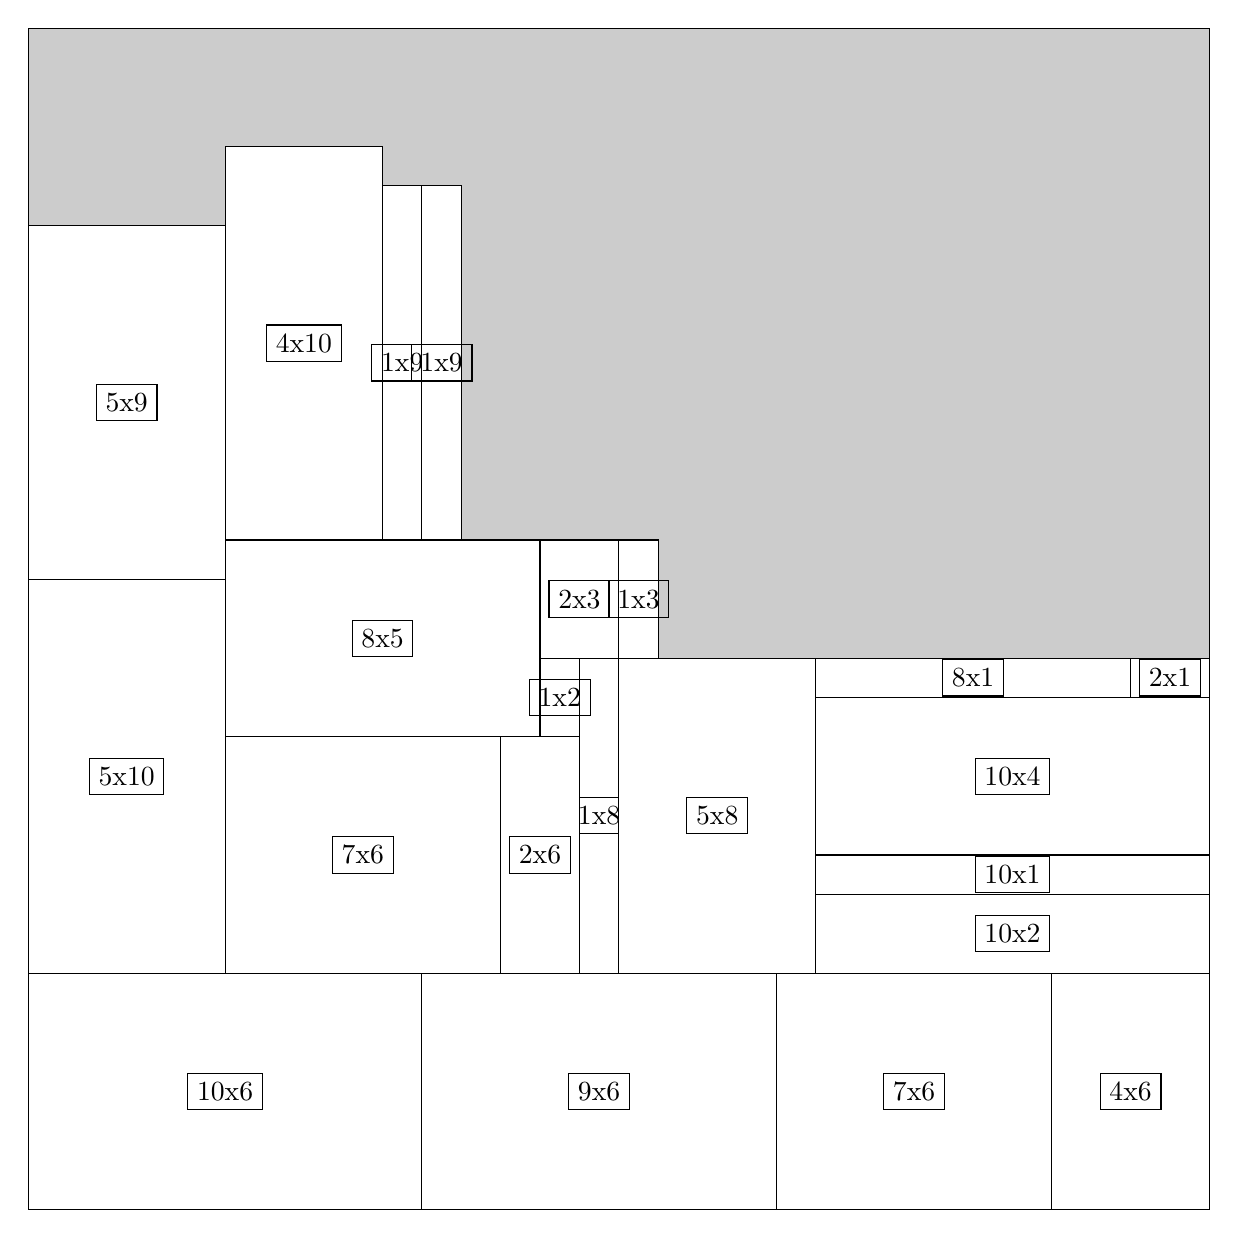
\begin{tikzpicture}[shorten >=1pt,scale=1.0,every node/.style={scale=1.0},->]
\tikzstyle{vertex}=[circle,fill=black!25,minimum size=14pt,inner sep=0pt]
\filldraw[fill=gray!40!white, draw=black] (0,0) rectangle (15.0,15.0);
\foreach \name/\x/\y/\w/\h in {10x6/0.0/0.0/5.0/3.0,9x6/5.0/0.0/4.5/3.0,5x10/0.0/3.0/2.5/5.0,5x9/0.0/8.0/2.5/4.5,7x6/9.5/0.0/3.5/3.0,7x6/2.5/3.0/3.5/3.0,1x8/7.0/3.0/0.5/4.0,8x5/2.5/6.0/4.0/2.5,5x8/7.5/3.0/2.5/4.0,4x10/2.5/8.5/2.0/5.0,4x6/13.0/0.0/2.0/3.0,10x2/10.0/3.0/5.0/1.0,2x6/6.0/3.0/1.0/3.0,10x1/10.0/4.0/5.0/0.5,1x9/4.5/8.5/0.5/4.5,1x9/5.0/8.5/0.5/4.5,8x1/10.0/6.5/4.0/0.5,10x4/10.0/4.5/5.0/2.0,2x3/6.5/7.0/1.0/1.5,1x3/7.5/7.0/0.5/1.5,2x1/14.0/6.5/1.0/0.5,1x2/6.5/6.0/0.5/1.0}
\filldraw[fill=white!40!white, draw=black] (\x,\y) rectangle node[draw] (\name) {\name} ++(\w,\h);
\end{tikzpicture}


w =10 , h =6 , x =0 , y =0 , v =60
\par
w =9 , h =6 , x =10 , y =0 , v =54
\par
w =5 , h =10 , x =0 , y =6 , v =50
\par
w =5 , h =9 , x =0 , y =16 , v =45
\par
w =7 , h =6 , x =19 , y =0 , v =42
\par
w =7 , h =6 , x =5 , y =6 , v =42
\par
w =1 , h =8 , x =14 , y =6 , v =8
\par
w =8 , h =5 , x =5 , y =12 , v =40
\par
w =5 , h =8 , x =15 , y =6 , v =40
\par
w =4 , h =10 , x =5 , y =17 , v =40
\par
w =4 , h =6 , x =26 , y =0 , v =24
\par
w =10 , h =2 , x =20 , y =6 , v =20
\par
w =2 , h =6 , x =12 , y =6 , v =12
\par
w =10 , h =1 , x =20 , y =8 , v =10
\par
w =1 , h =9 , x =9 , y =17 , v =9
\par
w =1 , h =9 , x =10 , y =17 , v =9
\par
w =8 , h =1 , x =20 , y =13 , v =8
\par
w =10 , h =4 , x =20 , y =9 , v =40
\par
w =2 , h =3 , x =13 , y =14 , v =6
\par
w =1 , h =3 , x =15 , y =14 , v =3
\par
w =2 , h =1 , x =28 , y =13 , v =2
\par
w =1 , h =2 , x =13 , y =12 , v =2
\par
\newpage


\end{document}